%-*-latex-*-
An interval is a collection of all real numbers between two given numbers. For
instance the closed interval $[1.2, 3.7]$ includes all the numbers between
$1.2$ and $3.7$, including $1.2$ and $3.7$.

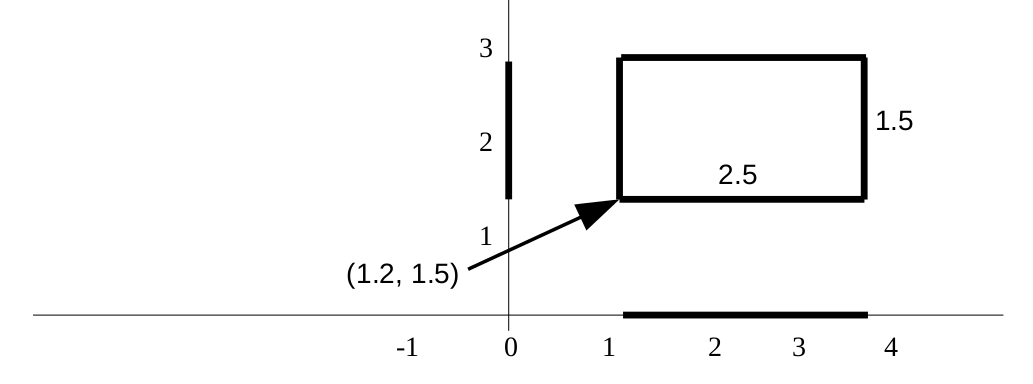
\includegraphics[width=6in, height=1in]{figure1.png}

Write a program that prompts the user for four numbers where the first two are 
the end points of a closed interval and the next two numbers are the end points
 of another interval. The program prints \verb!1! if the two intervals overlap,
and \verb!0! if the two intervals do not overlap.

For instance, the above interval $[1.2, 3.7]$ does not overlap with
$[5.0, 6.0]$. Hence this is an execution of the program:
\begin{console}[commandchars=\\\{\}]
\underline{1.2 3.7 5.0 6.0}
0
\end{console}

However, note that $[1.2, 3.7]$ overlaps with $[2.5, 4.0]$ since $3$ is in both
intervals.


\includegraphics[width=5.5in, height=0.75in]{figure2.png}

\resett
\nextt
\begin{console}[commandchars=\\\{\}]
\userinput{1.2 2.3 3.4 4.5}
0
\end{console}

\nextt
\begin{console}[commandchars=\\\{\}]
\userinput{3.4 4.5 1.2 2.3}
0
\end{console}

\nextt
\begin{console}[commandchars=\\\{\}]
\userinput{1.2 3.4 3.4 10}
1
\end{console}

\nextt
\begin{console}[commandchars=\\\{\}]
\userinput{1.2 3.4 3 10}
1
\end{console}

\nextt
\begin{console}[commandchars=\\\{\}]
\userinput{1.2 3.4 0 10}
1
\end{console}

\nextt
\begin{console}[commandchars=\\\{\}]
\userinput{3.4 10 1.2 3.4}
1
\end{console}

\nextt
\begin{console}[commandchars=\\\{\}]
\userinput{3 10 1.2 3.4}
1
\end{console}

\nextt
\begin{console}[commandchars=\\\{\}]
\userinput{0 10 1.2 3.4}
1
\end{console}

(This is very important for collision detection in computer games,
at least for very simple games. You need a more powerful algorithm
for high-end games.)
